\section{CDM simulations}
\label{sec:cdm-sim}

\subsection{Initial galaxy equilibration}
Before simulating the Sgr infall, we evolved the MW and Sgr galaxies
individually for 10 Gyr such that each galaxy would be equilibrated. This is
done to ensure that any dynamical phenomena occuring during the Sgr infall is a
result of MW-Sgr interactions and not due to local inequilibria. Given that the
initial distributions of stellar and DM particles follow distributions which are
supposed to be near-equilibrium, little change is expected during these
preliminary simulations.

Interestingly, however, the galaxies show a tendency to redistribute halo mass
away from the center of the halo during the first few Gyr of evolution. This is
matched by a changing disk density distribution; as such, we believe this
phenomenon to be the result of interaction between the halo and disk
gravitational potentials. This phenomenon appears to be in line with similar
trends found for gas disks in~\cite{deg_galactics_2019}.

Plots of the evolutions of the mass distributions for the MW and Sgr halos are
shown in Figure~\ref{fig:cdm_init_halo}, where the reference NFW distributions
from equation~\ref{eq:halo_dist} are also plotted. While the effects of this
phenomenon are unlikely to cause significant disruptions to our future
results, it is an important deviation from the NFW distribution.

\begin{figure}[t]
    \centering
    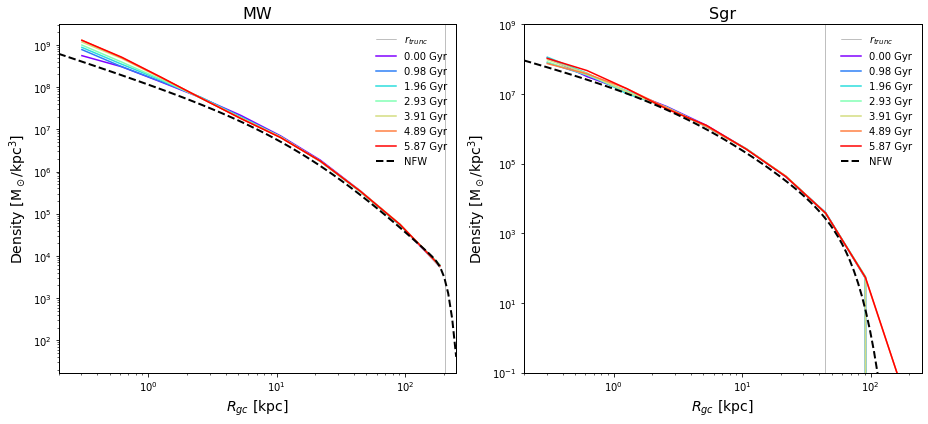
\includegraphics[width=0.9\linewidth]{fig/cdm/init_halo.png}
    \caption{
        Plotted are the halo mass density distributions for the MW (left) and
        Sgr (right) galaxies during their initial, independent equilibration
        evolutions. Also plotted are the reference NFW distributions (dashed
        black line), following equation~\ref{eq:halo_dist} \textit{with} the
        truncation function (equation~\ref{eq:trunc}) included, and the
        truncation radius (vertical grey line).
    }
    \label{fig:cdm_init_halo}
\end{figure}

The evolution of the mass distributions for the MW and Sgr disks are shown in
Figure~\ref{fig:cdm_init_disk}. Here, the reference distribution, given in
equation~\ref{eq:disk_dist}, is also plotted. We see an interesting trend in the
evolution of the Sagittarius disk where mass is redistributed outward to radii
significantly beyond the truncation radius. This could be an indication that we
need to consider a larger value of $r_t$ so that such large changes are not
needed to obtain equilibrium.

\begin{figure}[t]
    \centering
    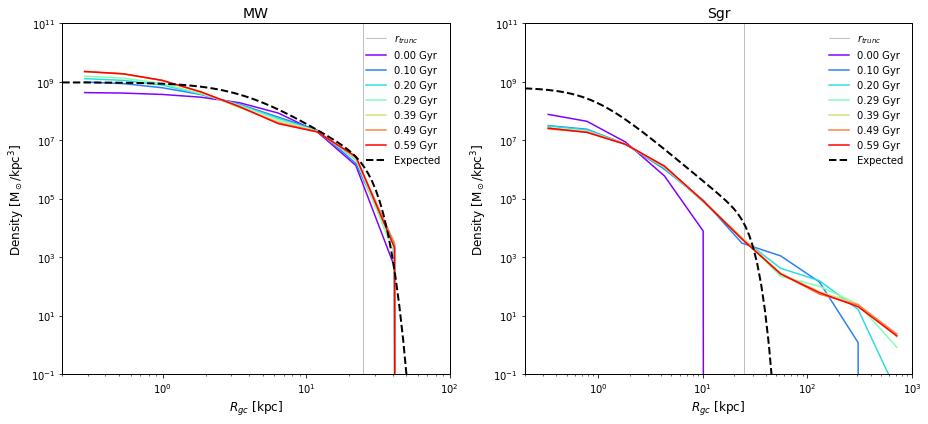
\includegraphics[width=0.9\linewidth]{fig/cdm/init_disk.png}
    \caption{
        Plotted are the disk mass density distributions for the MW (left) and
        Sgr (right) galaxies during their initial, independent equilibration
        evolutions. Also plotted are the reference distributions (dashed black
        line), following equation~\ref{eq:disk_dist} \textit{with} the
        truncation function (equation~\ref{eq:trunc}) included, and the
        truncation radius (vertical grey line).
    }
    \label{fig:cdm_init_disk}
\end{figure}

\subsection{Sgr infall evolution}
With the MW and Sgr galaxies equilibrated, we merge the particles of these
galaxies, placing the MW at rest at the origin and the Sgr progenitor at
$\vec{r} = (125, 0, 0)$ kpc with an initial velocity of $\vec{v} = (-10, 0, 70)$
km s$^{-1}$, following~\cite{dierickx_predicted_2017}. The resulting merged
galaxies are then evolved for roughly 10 Gyr. 

The evolution of the mass density distributions of the MW galaxy is shown in
Figure~\ref{fig:cdm_merged_mw}. We can see that the halo distribution, while
deviating away from the reference NFW distribution at low radii, remains stable
throughout the evolution, implying that it had truly reached equilibrium in our
previous run despite its disagreement with the reference distribution. The disk
distribution also appears to remain quite stable, with the only notable changes
occuring a large radii where interactions with Sgr are likely.

\begin{figure}[h]
    \centering
    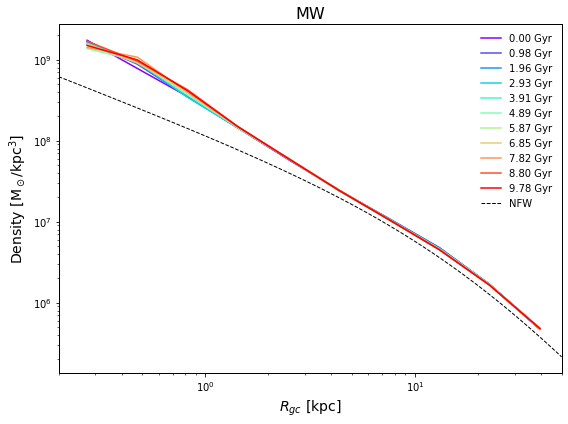
\includegraphics[width=0.45\linewidth]{fig/cdm/merged_mw_halo.png}
    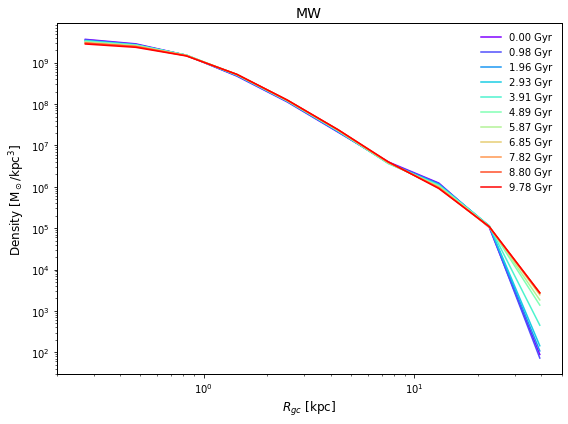
\includegraphics[width=0.45\linewidth]{fig/cdm/merged_mw_disk.png}
    \caption{
        The halo (left) and disk (right) mass density distributions for the MW
        galaxy in the merged evolution of the MW and Sgr galaxies. The reference
        NFW distribution is also plotted for the halo distribution. The halo
        distribution remains remarkably constant, even in the low radius
        region where there is high deviation from the NFW distribution. The disk
        distribution also remains quite constant, with the only strong changes
        occuring at high radii, near the Sgr galaxy.
    }
    \label{fig:cdm_merged_mw}
\end{figure}

We can track the trajectory of the center of stellar mass of the Sgr galaxy
during its infall as well. Note that this is only strongly accurate for the
first few Gyr, as each tidal stripping during each orbit of the MW results in
a much more disparate spread of Sgr stars after several Gyr. The trajectory is
shown in Figure~\ref{fig:cdm_merged_sgr}. Compared
to~\cite{dierickx_predicted_2017} (e.g. their Figure 6), our model shows a
significantly less smooth infall trajectory with less strongly oscillatory
behavior in the separation distance. 

\begin{figure}[h!]
    \centering
    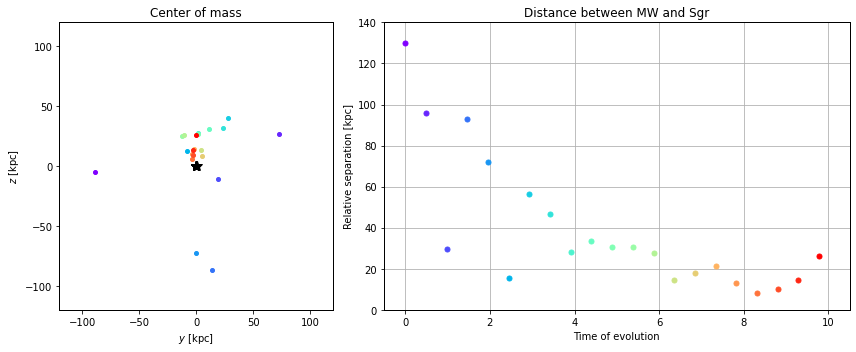
\includegraphics[width=0.9\linewidth]{fig/cdm/merged_trajectory.png}
    \caption{
        The trajectory of the Sgr center of stellar mass during its infall into
        the MW. Plotted on the left are the centers of stellar mass of the MW
        (black star) and Sgr (colored circles) over time. Plotted on the right
        is the separation distance between the MW and Sgr. 
    }
    \label{fig:cdm_merged_sgr}
\end{figure}

Also following~\cite{dierickx_predicted_2017}, we compute the observational
coordinates of the simulated Sgr center-of-mass and compare to the actual
observed coordinates (e.g. compare to their Figure 7). The observed
coordinates are given as follows:

\begin{itemize}
    \item $(\text{RA}, \text{dec}) = (283.83, -29.45)$
    deg~\cite{nasa_nasaipac_nodate}
    \item $\text{Heliocentric distance} = 24.8 \pm 0.8$
    kpc~\cite{kunder_distance_2009}
    \item $(\mu_{\alpha} \cos\delta, \mu_{\delta}) = (-2.54 \pm 0.18, -1.19 \pm 0.16)$ mas/yr~\cite{massari_hubble_2013}
    \item $\langle V_r \rangle \text{(radial velocity)} = 139.4 \pm 0.6$ km/s~\cite{bellazzini_nucleus_2008}
\end{itemize}

The results are plotted in Figure~\ref{fig:cdm_merged_coords}.
None of our simulation snapshots attain similar coordinates to the observed
coordinates, unlike~\cite{dierickx_predicted_2017}. Solving these
discrepancies will likely require re-simulation or better time resolution in
our analysis.

\begin{figure}[t]
    \centering
    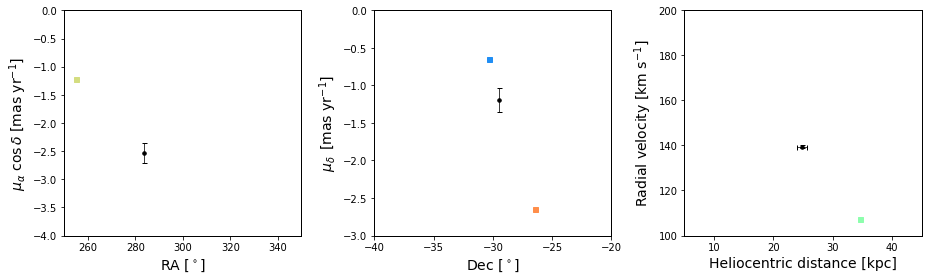
\includegraphics[width=0.9\linewidth]{fig/cdm/merged_obs_coords.png}
    \caption{
        The observed coordinates of Sgr as well as the coordinates of the
        simulated Sgr in our snapshots. Axis limits are set such that only
        snapshots with reasonably-close values to the accepted observations are
        shown. No single snapshot falls within these ranges for more than one of
        the plotted coordinate pairs. Observed coordinates come
        from~\cite{nasa_nasaipac_nodate,kunder_distance_2009,massari_hubble_2013,bellazzini_nucleus_2008}.
    }
    \label{fig:cdm_merged_coords}
\end{figure}

The above plots allow us to conclude that our simulation did not yield any
best-fit snapshots that were remarkably similar to the position of Sgr today. As
such, it is difficult to draw quantitative conclusions about the stream today.
However, the resulting stream qualitatively agrees well with the results of
other models, such as~\cite{dierickx_predicted_2017}. See
Figures~\ref{fig:cdm_merged_stars} and~\ref{fig:cdm_merged_dm} for
illustrations of the Sgr star and dark matter particles over time.

\begin{figure}[t]
    \centering
    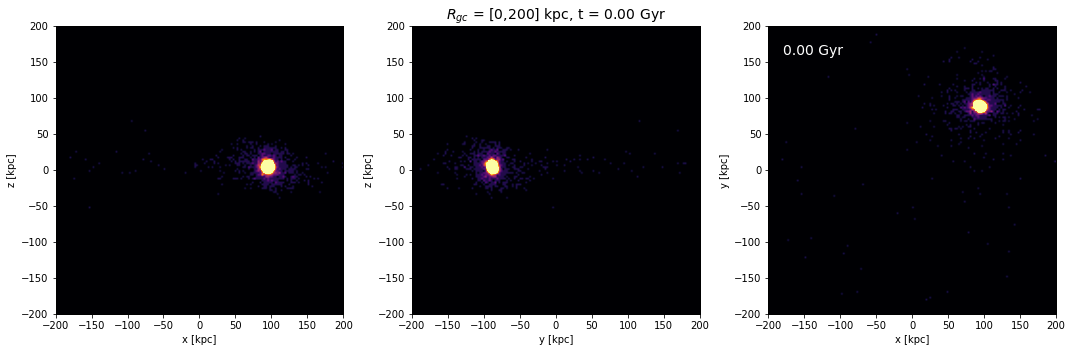
\includegraphics[width=0.9\linewidth]{fig/cdm/merged_star_0.png}
    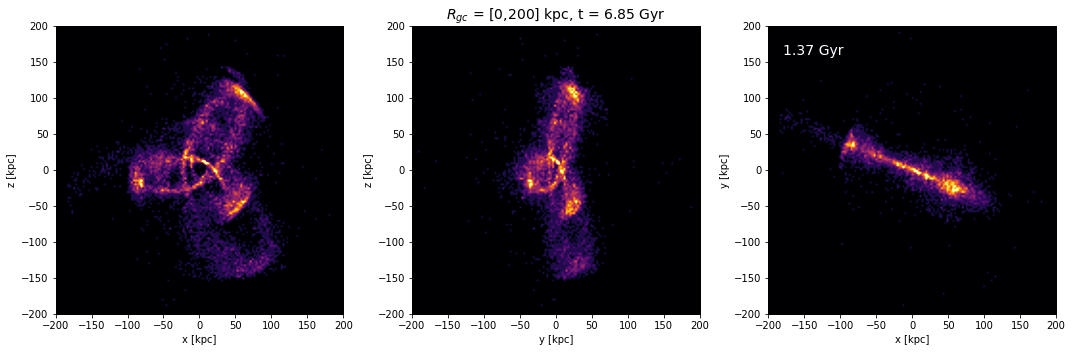
\includegraphics[width=0.9\linewidth]{fig/cdm/merged_star_685.png}
    \caption{
        The positions of the the Sgr star particles at 0 Gyr of evolution
        (top) and 6.85 Gyr of evolution (bottom). These plots qualitatively
        agree with expected results, showing the triaxial stream distribution.
    }
    \label{fig:cdm_merged_stars}
\end{figure}

\begin{figure}[t]
    \centering
    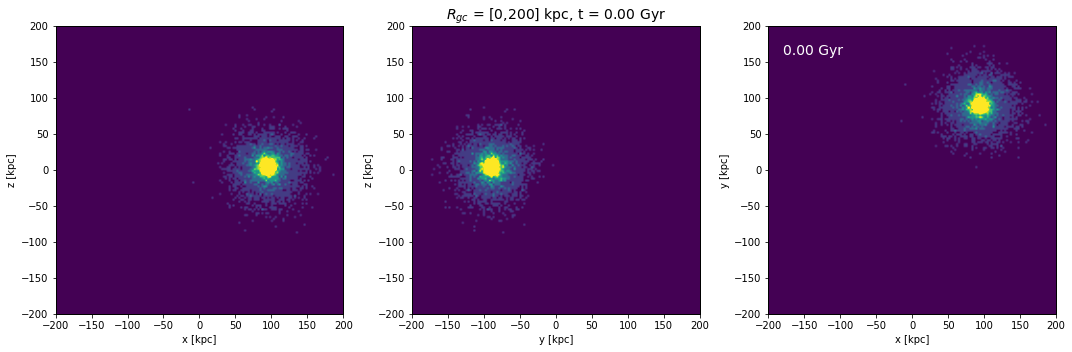
\includegraphics[width=0.9\linewidth]{fig/cdm/merged_dm_0.png}
    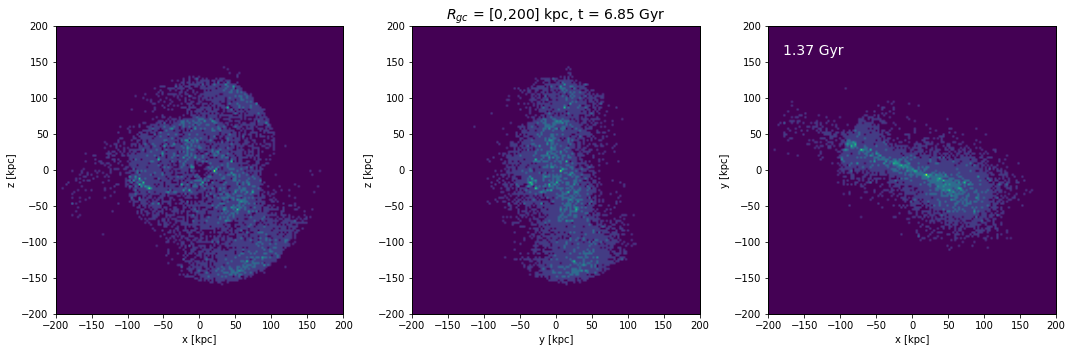
\includegraphics[width=0.9\linewidth]{fig/cdm/merged_dm_685.png}
    \caption{
        The positions of the the Sgr dark matter particles at 0 Gyr of evolution
        (top) and 6.85 Gyr of evolution (bottom). These plots qualitatively
        agree with expected results, showing the triaxial stream distribution.
    }
    \label{fig:cdm_merged_dm}
\end{figure}
